\section{SHEAR STRENGTH AND N-VALUE 抗剪强度和N值}

\begin{paracol}{2}
    
    Now that the relation between shear modulus $G_0$ and N-value of the standard penetration test has been evaluated in the preceding section, the relation between shear strength $S_u$ and N-value has to be evaluated, too, in a similar way.

    Shear strength $S_u$ can be obtained from \autoref{equation:8} by use of the results of triaxial compression test on undisturbed soil samples. When the relation between shear strength and N-value is to be evaluated, particular attention has to be paid to soil sampling practice and accuracy of soil test. With this taken into account, the authors have sampled data solely from such basic soil exploration reports as considered to be under stringent supervision for securing as high accuracy as possible of soil test and, especially, the results of such soil tests as were conducted with special attention paid to sampling method\citep{Koizumi1968} or by use of block samples, since soil samples are easy to be disturbed, if N-value exceeds 10.

    \switchcolumn

    现在,在上一节中已经评估了剪切模量$G_0$与标准渗透试验的N值之间的关系,因此也必须以类似的方式评估剪切强度$S_u$与N值之间的关系。
        
    抗剪强度$S_u$可以使用\cnequationref{equation:8}的三轴压缩试验结果在未经扰动的土体样品上获得。 当要评估抗剪强度与N值之间的关系时,必须特别注意土体取样和土体试验的准确性。 考虑到这一点,作者仅从基本的土体勘探报告中取样数据,这些报告被认为受到严格的监督,以确保尽可能高的土体测试准确性,尤其是在特殊条件下进行的土体测试结果 注意如果N值超过10,土体样本很容易受到干扰,请注意抽样方法\citep{Koizumi1968}或使用块状样本。

\end{paracol}

\Paragraph{Criteria of Data Sampling 数据采样标准}

\begin{paracol}{2}
    
    Criteria of data sampling was set up so that the following requirements could be satisfied :
    \begin{enumerate}
        \item Soil has to fall under the category of cohesive soil.
        \item Soil sampling and standard penetration test have to be carried out in the same borehole.
        \item Any data with N-value of less than 1.0 shall be rejected, because there exists no coefficient of correlation between shear strength and N-value, if the latter is less than 1.0.
    \end{enumerate}
    \switchcolumn

    建立了数据采样标准,以便满足以下要求:
    \begin{enumerate}
        \item 土样必须属于黏性土体。
        \item 必须在同一钻孔中进行土体取样和标准渗透试验。
        \item 任何N值小于1.0的数据均应被拒绝,因为如果N值小于1.0,则抗剪强度与N值之间不存在相关系数。
    \end{enumerate}
    
\end{paracol}

\Paragraph{Relation between Shear Strength and N-Value 抗剪强度与N值的关系}

\begin{paracol}{2}
    
    Just as in the preceding section, the data on shear strength and N-value thus sampled are plotted on a logarithmic graph shown in \autoref{figure:12}. On the assumption that the first order equation should be $S_u=aN^b$, the following empirical formula was obtained by calculating $a$ and $b$ the method of least squares :

    \switchcolumn

    与前面的部分一样,将这样取样的抗剪强度和N值数据绘制在\cnfigureref{figure:12}所示的对数图上。假设一阶方程应为$S_u=aN^b$,则可通过以下公式获得以下经验公式:计算$a$和$b$的最小二乘法:

\end{paracol}

\begin{align}
    S_u=0.297N^{0.72}(\rm{kg/cm^2})
    \label{equation:11}
\end{align}
\begin{figure*}[!htb]
    \begin{minipage}[t]{0.48\textwidth}
        \centering
        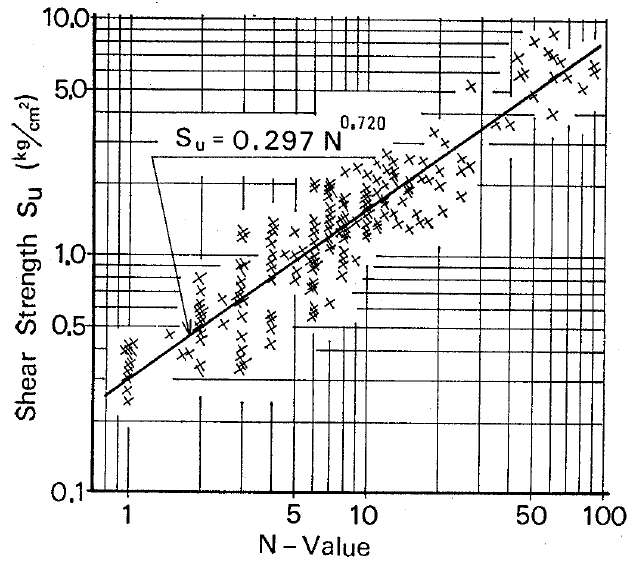
\includegraphics[width=\textwidth]{figures/figure-12.png}
        \caption{Relationship between $S_u$ and N-value}
        \addtocounter{figure}{-1}
        \vspace{-5pt}
        \renewcommand{\figurename}{图}
        \caption{$S_u$和N值之间的关系}
        \renewcommand{\figurename}{Figure}
        \label{figure:12}
    \end{minipage}
    \begin{minipage}[t]{0.48\textwidth}
        \centering
        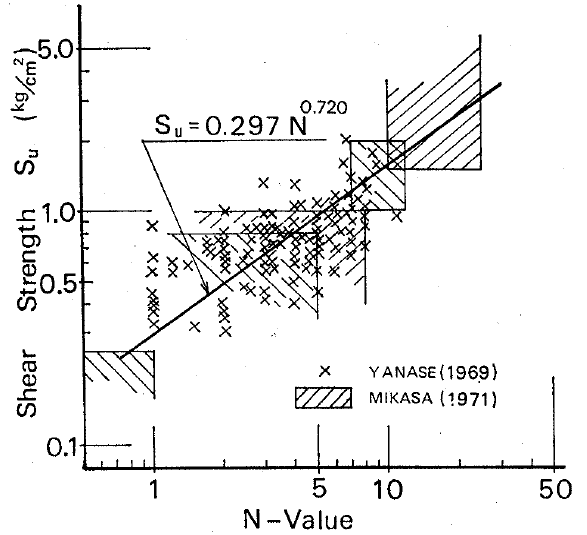
\includegraphics[width=\textwidth]{figures/figure-13.png}
        \caption{Comparison between \autoref{equation:11} and similar data by others}
        \addtocounter{figure}{-1}
        \vspace{-5pt}
        \renewcommand{\figurename}{图}
        \caption{\autoref{equation:11}与其他类似数据之间的比较}
        \renewcommand{\figurename}{Figure}
        \label{figure:13}
    \end{minipage}
\end{figure*}


\begin{paracol}{2}

    \noindent{}where coefficient of correlation $\rho_{xy}=0.93$.

    \switchcolumn      
     
    \noindent{}其中相关系数$\rho_{xy}=0.93$。

\end{paracol}

\Paragraph{Comparison with Other Investigations 与其他调查研究的比较}

\begin{paracol}{2}
    

    The shear strength of clay can be approximately obtained from the unconfined compression strength $q_u$ by the following equation.

    \switchcolumn

    黏土的剪切强度可以通过以下等式从无侧限抗压强度$q_u$近似获得。

\end{paracol}

\begin{align}
    S_u\doteq\frac{1}{2}q_u(\rm{kg/m^2})
\end{align}

\begin{paracol}{2}

    \citet{Mikasa197138} has shown the range of N-value and unconfined compression strength of cohesive soil on the basis of his investigation into typical cohesive soil layers in Osaka district. Similarly, \citet{Yanase196937} has shown many data on N-value and unconfined compression strength of cohesive soil by way of his test conducted on such soil samples as considered to have been least disturbed during sampling. These data are plotted in \autoref{figure:13} together with graphical expression of \autoref{equation:11}, which is expressed as a straight line passing near the center of those data shown by Mikasa\citet{Mikasa197138} and Yanase\citet{Yanase196937}.

    \switchcolumn

    \citet{Mikasa197138}在对大阪地区典型的黏性土层进行调查的基础上,显示了黏性土的N值范围和无侧限抗压强度。 同样,\citet{Yanase196937}通过对这样的土壤样本进行的测试,显示出许多关于黏性土壤的N值和无侧限抗压强度的数据,这些样本被认为在采样过程中受到的干扰最小。 这些数据与\cnequationref{equation:11}的图形表达式一起绘制在\cnfigureref{figure:13}中,该等式表示为一条直线,通过的直线靠近Mikasa\citet{Mikasa197138}和Yanase\citet{Yanase196937}展示的那些数据的中心。

\end{paracol}